\documentclass[11pt,a4paper]{article}
\usepackage[margin=2.2cm]{geometry}
\usepackage{amsmath,graphicx,booktabs,float,hyperref}
\title{Ringdown of a black hole surrounded by a thin shell of matter:\\ a reanalysis with Advanced LIGO noise}
\author{Darin La Rocca\\ \small University of Milano-Bicocca}
\date{\today}
\begin{document}
\maketitle

\section{Goal}
This note reanalyses the public waveforms of Laeuger, Weller, Li \& Chen, \emph{The ringdown of a black hole
surrounded by a thin shell of matter}, arXiv:2506.00367 (data: Zenodo, DOI 10.5281/zenodo.15586889).
The question is whether a fit of the ringdown can tell a black hole with a shell of matter apart from a
black hole in vacuum, and whether this still holds with realistic detector noise. The paper itself does not
include detector noise; the last test (Advanced LIGO noise) is an extension of this work.
Three shell configurations are studied in detail. Then, to see the trend with the mass and the radius of the shell,
the Advanced LIGO test is repeated on all twelve shell configurations of the data set.

\section{Data and method}
Three shell configurations are studied (Table~\ref{tab:cases}). The code uses $M=0.5$; below, times are in
units of $M$ and frequencies are given as $M\omega$. Each fit uses a window that starts $10M$ after the peak
of the signal.

As a check of units, the data set also contains the fundamental mode computed by the authors for a
shell of zero mass, $M\omega=0.373672-0.088962i$, which agrees with the value of Berti, Cardoso \&
Starinets used here ($0.373672-0.088962i$).

\begin{table}[H]
\centering\footnotesize
\begin{tabular}{llccccc}
\toprule
Case & Shell & $\delta M/M$ & $R/M$ & $\alpha$ & Window [$M$] & Shell modes \\
\midrule
Case 1 & heavy, close shell (dM = M/2, R = 6M) & 0.5 & 6 & 1.1547 & 10-200 & 2 \\
Case 2 & light, distant shell (dM = M/100, R = 30M) & 0.01 & 30 & 1.0004 & 10-135 & 8 \\
Case 3 & heavy, distant shell (dM = M/2, R = 30M) - echo & 0.5 & 30 & 1.0184 & 10-135 & 9 \\
\bottomrule
\end{tabular}
\caption{Shell configurations. $\alpha=\sqrt{(1-2M/R)/(1-2(M+\delta M)/R)}$ is the redshift factor between the inside of the shell and infinity (eq.~17 of the paper).\label{tab:cases}}
\end{table}


\paragraph{1. Fixed-mode fits.} The signal is fitted with $N=1,\dots,4$ damped sinusoids
whose complex frequencies $\omega_k$ are fixed,
\begin{equation}
h(t)\simeq\sum_k e^{\mathrm{Im}\,\omega_k t}\left[a_k\cos(\mathrm{Re}\,\omega_k t)+b_k\sin(\mathrm{Re}\,\omega_k t)\right],
\end{equation}
and the amplitudes $a_k,b_k$ are found by linear least squares. Three sets of frequencies are compared:
the Schwarzschild $\ell=2$ modes $n=0,\dots,3$ (Berti, Cardoso \& Starinets 2009), the shell modes as listed in
the data files, and the shell modes divided by $\alpha$. As in the paper, at most four modes are used, the
least damped ones for the shell. The quality of a fit is the mismatch (eqs.~30--31 of the paper)
\begin{equation}
\mathcal{M}=1-\frac{\langle h,h_\mathrm{fit}\rangle}{\sqrt{\langle h,h\rangle\langle h_\mathrm{fit},h_\mathrm{fit}\rangle}},
\qquad \langle a,b\rangle=\int_{t_0}^{t_1}a\,b\,dt .
\end{equation}

\paragraph{2. Free fit.} 2 damped sinusoids $A\,e^{-\gamma t}\cos(\omega t+\varphi)$ with
free $\omega$ and $\gamma$ are fitted (several starting points, best fit kept). Each fitted frequency
$\omega-i\gamma$ is compared with the closest mode of each set.

\paragraph{3. Bias test.} The same free fit is repeated on a synthetic signal built only from vacuum modes.
Any deviation from the vacuum modes found here is produced by the method, not by the shell.

\paragraph{4. Advanced LIGO noise.} To use detector noise, a physical mass is needed: $M=60\,M_\odot$, so that $1M=0.30$\,ms and the fundamental vacuum
mode is at $201$\,Hz. Gaussian noise is drawn from the Advanced LIGO
design sensitivity (PyCBC, \texttt{aLIGOZeroDetHighPower}, $f>20$\,Hz). The signal on the
fit window is rescaled to an optimal SNR $\rho=\sqrt{\langle h,h\rangle}$, and both the fits and the mismatch
use the noise-weighted inner product
\begin{equation}
\langle a,b\rangle=4\,\mathrm{Re}\int_{f_\mathrm{low}}^{\infty}\frac{\tilde a(f)\,\tilde b^*(f)}{S_n(f)}\,df .
\end{equation}
For each SNR, 100 noise realizations are generated and the fraction in which the shell
modes give a lower $\chi^2$ than the vacuum modes is recorded. To compare models with the same number of free
parameters, both use $n=\min(4,N_\mathrm{shell})$ modes: the $n$ lowest vacuum overtones against the $n$ shell
modes (divided by $\alpha$) that are most excited in the signal, i.e.\ with the largest amplitude when all the
listed shell modes are fitted together to the noiseless waveform (the fraction with a lower
noise-weighted mismatch is also saved, and gives the same result).

\section{Results}
\subsection{Fixed-mode fits}

\begin{table}[H]
\centering\small
\begin{tabular}{lccccc}
\toprule
Case & vacuum & shell (as listed) & shell / $\alpha$ & vacuum, $10$--$100M$ & shell / $\alpha$, $10$--$100M$ \\
\midrule
Case 1 & $2.04\times10^{-2}$ (4) & $6.21\times10^{-2}$ (2) & \textbf{$1.08\times10^{-4}$} (2) & $1.49\times10^{-2}$ & $1.06\times10^{-4}$ \\
Case 2 & \textbf{$6.99\times10^{-6}$} (4) & $2.14\times10^{-5}$ (4) & $2.13\times10^{-5}$ (4) & $6.49\times10^{-6}$ & $2.08\times10^{-5}$ \\
Case 3 & $1.14\times10^{-3}$ (4) & \textbf{$5.79\times10^{-4}$} (4) & $7.13\times10^{-4}$ (4) & $1.09\times10^{-3}$ & $7.11\times10^{-4}$ \\
\bottomrule
\end{tabular}
\caption{Mismatch with $N=4$ requested modes (number actually used in brackets) on the fit window, and on the window of the paper ($10M$--$100M$). Best set in bold.}
\end{table}

\begin{figure}[H]
\centering
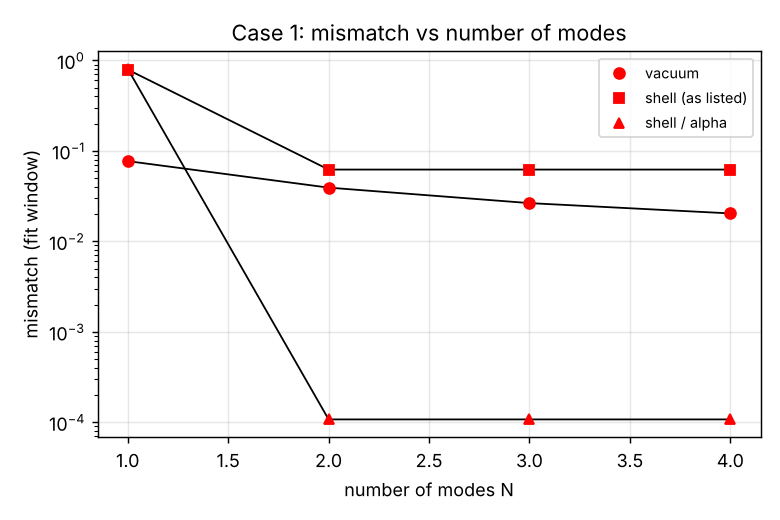
\includegraphics[width=0.32\linewidth]{plots/case_1_mismatch.png}
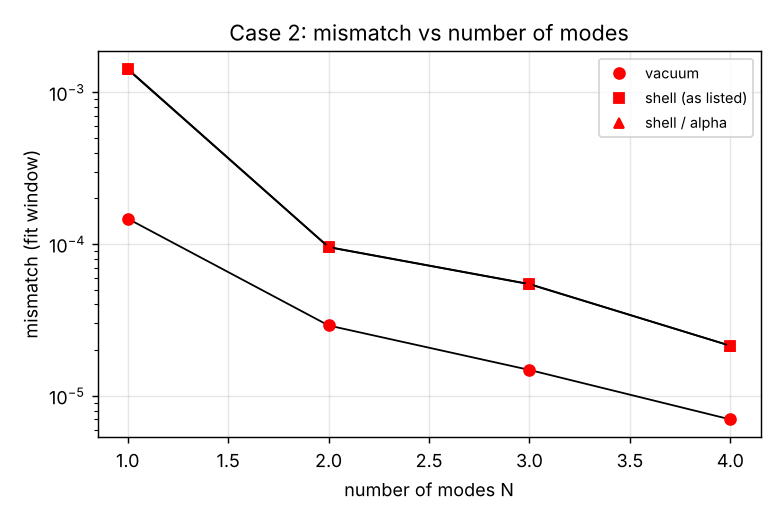
\includegraphics[width=0.32\linewidth]{plots/case_2_mismatch.png}
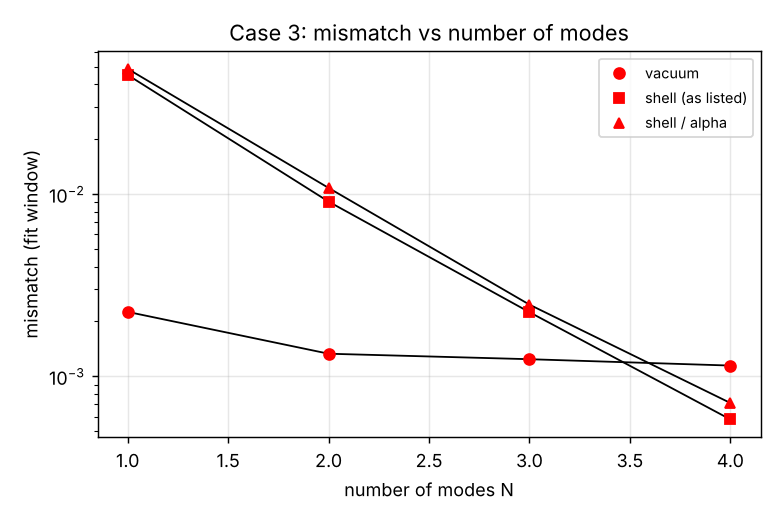
\includegraphics[width=0.32\linewidth]{plots/case_3_mismatch.png}
\caption{Mismatch as a function of the number of modes.}
\end{figure}

\begin{figure}[H]
\centering
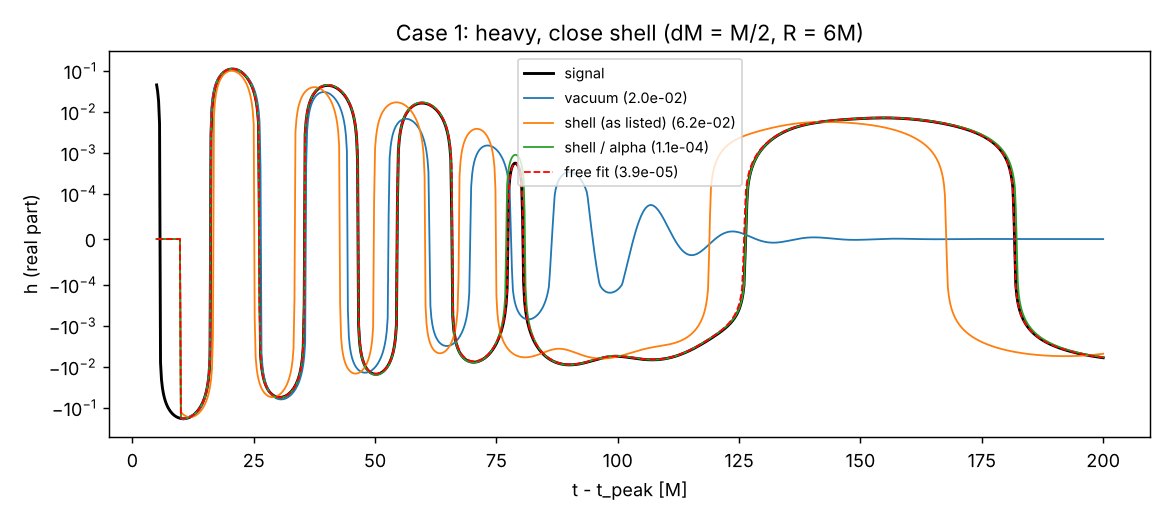
\includegraphics[width=0.85\linewidth]{plots/case_1_fits.png}
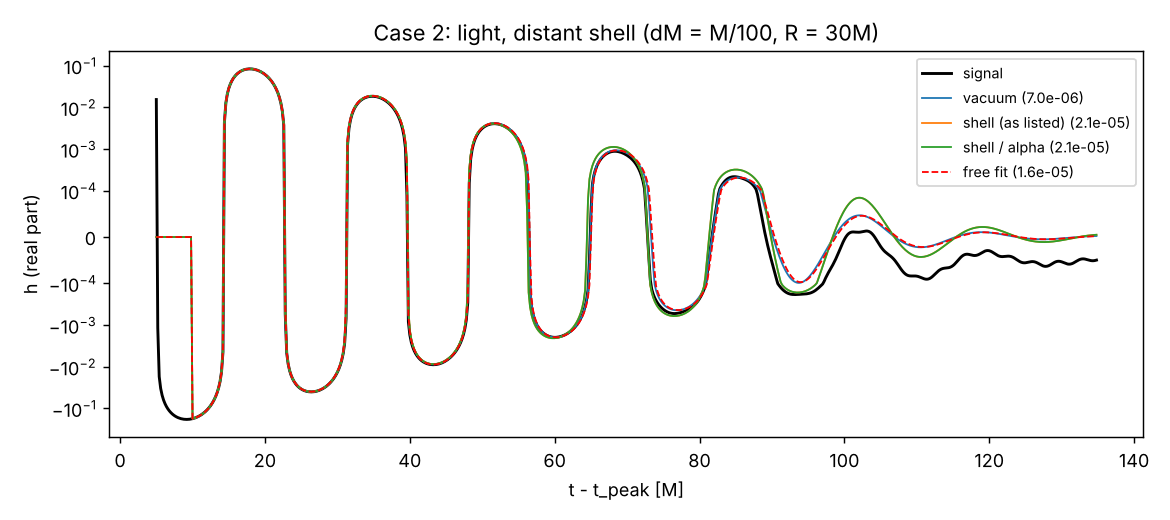
\includegraphics[width=0.85\linewidth]{plots/case_2_fits.png}
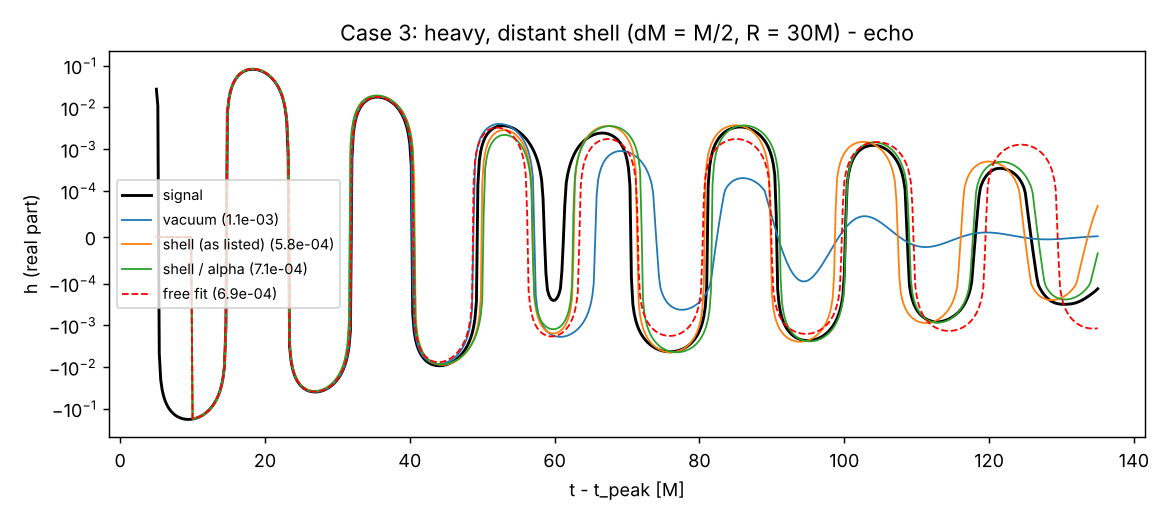
\includegraphics[width=0.85\linewidth]{plots/case_3_fits.png}
\caption{Signal and best fits with $N=4$ modes (mismatch in the legend).}
\end{figure}

\subsection{Free fit and bias test}

\begin{table}[H]
\centering\small
\begin{tabular}{lccccc}
\toprule
Case & Mode & $M\omega$ & $M\gamma$ & Closest set & $\mathcal{M}$ of free fit \\
\midrule
Case 1 & 1 & 0.3188 & 0.0547 & shell / $\alpha$ & $3.87\times10^{-5}$ \\
Case 1 & 2 & 0.0560 & 0.0000 & shell / $\alpha$ & $3.87\times10^{-5}$ \\
Case 2 & 1 & 0.3718 & 0.0890 & vacuum & $1.59\times10^{-5}$ \\
Case 2 & 2 & 0.5740 & 0.2767 & shell (as listed) & $1.59\times10^{-5}$ \\
Case 3 & 1 & 0.3651 & 0.0843 & vacuum & $6.86\times10^{-4}$ \\
Case 3 & 2 & 0.3153 & 0.0055 & shell (as listed) & $6.86\times10^{-4}$ \\
\bottomrule
\end{tabular}
\caption{Free fit: fitted frequency and damping, and the closest set of modes.}
\end{table}

\begin{table}[H]
\centering\small
\begin{tabular}{lcccccc}
\toprule
Case & Mode & $M\omega$ fitted & $M\gamma$ fitted & $M\omega$ vacuum & $M\gamma$ vacuum & Distance ($M|\Delta\omega|$) \\
\midrule
Case 1 & 1 & 0.2916 & 0.0889 & 0.3737 & 0.0890 & 0.0820 \\
Case 1 & 2 & 0.3761 & 0.0498 & 0.3737 & 0.0890 & 0.0392 \\
Case 2 & 1 & 0.3714 & 0.0885 & 0.3737 & 0.0890 & 0.0023 \\
Case 2 & 2 & 0.6523 & 0.3972 & 0.3467 & 0.2739 & 0.3295 \\
Case 3 & 1 & 0.3666 & 0.0899 & 0.3737 & 0.0890 & 0.0071 \\
Case 3 & 2 & 0.4658 & 0.1176 & 0.3737 & 0.0890 & 0.0965 \\
\bottomrule
\end{tabular}
\caption{Bias test: free fit on a vacuum-only signal, compared with the nearest vacuum mode.}
\end{table}

\subsection{Advanced LIGO noise}
For each case and SNR, 100 independent
realizations of Advanced LIGO noise are added to the signal and both fits (vacuum modes and shell modes) are
repeated on each of them. Table~\ref{tab:ligo} gives the fraction of realizations in which the shell modes give the
lower $\chi^2$. A value of 100\% means that the shell modes always describe the data better, so the shell is
clearly identified; a value around 50\% means that the outcome is random, as for a coin toss, so the two
hypotheses cannot be distinguished; a value below 50\% means that the vacuum modes are preferred. In the summary,
the shell is called distinguishable when its modes win in at least 90\% of the realizations.


\begin{table}[H]
\centering\small
\begin{tabular}{lccccc}
\toprule
Case & SNR 10 & SNR 30 & SNR 100 & SNR 300 & SNR 1000 \\
\midrule
Case 1 & 83 $\pm$ 4\% & 100 $\pm$ 0\% & 100 $\pm$ 0\% & 100 $\pm$ 0\% & 100 $\pm$ 0\% \\
Case 2 & 53 $\pm$ 5\% & 44 $\pm$ 5\% & 37 $\pm$ 5\% & 20 $\pm$ 4\% & 0 $\pm$ 0\% \\
Case 3 & 40 $\pm$ 5\% & 49 $\pm$ 5\% & 89 $\pm$ 3\% & 100 $\pm$ 0\% & 100 $\pm$ 0\% \\
\bottomrule
\end{tabular}
\caption{Fraction of the 100 noise realizations in which the shell modes fit better than the vacuum modes. Values near 50\% mean that the two cannot be distinguished.\label{tab:ligo}}
\end{table}

The fit with fixed modes is a noise-weighted least-squares fit, so its minimum is
$\chi^2=\langle d-h_\mathrm{fit},d-h_\mathrm{fit}\rangle$. The number of degrees of freedom is
$N_\mathrm{eff}-2N_\mathrm{modes}$, where $N_\mathrm{eff}$ is the mean of $\langle n,n\rangle$ over 300 pure-noise
realizations (the effective number of independent points). Table~\ref{tab:chi2} gives, for each SNR, the mean
$\chi^2/\mathrm{ndof}$ of the two fits with its $p$-value, and the difference $\Delta\chi^2=\chi^2_\mathrm{vac}-
\chi^2_\mathrm{shell}$. Since the two models have the same number of parameters, $\Delta\chi^2$ is twice the
log-likelihood ratio: positive values favour the shell. The two models are not nested, so no $p$-value is attached
to $\Delta\chi^2$; its mean and spread over the noise realizations are reported instead. The errors on the
fractions are binomial, $\sqrt{f(1-f)/N}$ (zero when $f$ is exactly 0 or 1).


\begin{table}[H]
\centering\small
\begin{tabular}{lccccccc}
\toprule
Case & SNR & $\chi^2/$ndof vac. & $p$ vac. & $\chi^2/$ndof shell & $p$ shell & $\Delta\chi^2$ (mean $\pm$ std) & lower $\mathcal{M}$ \\
\midrule
Case 1 & 10 & 1.00 & 0.45 & 1.00 & 0.5 & 5.9 $\pm$ 6.9 & 83\% \\
Case 1 & 30 & 1.05 & 0.14 & 1.00 & 0.53 & 50.1 $\pm$ 15.1 & 100\% \\
Case 1 & 100 & 1.64 & 5.2e-32 & 1.00 & 0.46 & 602.3 $\pm$ 53.3 & 100\% \\
Case 1 & 300 & 6.72 & 0 & 1.01 & 0.39 & 5431.5 $\pm$ 183.1 & 100\% \\
Case 1 & 1000 & 64.57 & 0 & 1.17 & 0.00024 & 60298.3 $\pm$ 483.0 & 100\% \\
Case 2 & 10 & 1.00 & 0.48 & 1.00 & 0.48 & -0.0 $\pm$ 3.9 & 53\% \\
Case 2 & 30 & 0.99 & 0.53 & 1.00 & 0.52 & -0.7 $\pm$ 3.0 & 44\% \\
Case 2 & 100 & 0.99 & 0.58 & 0.99 & 0.57 & -1.0 $\pm$ 3.4 & 37\% \\
Case 2 & 300 & 1.00 & 0.51 & 1.00 & 0.46 & -3.9 $\pm$ 5.4 & 20\% \\
Case 2 & 1000 & 1.00 & 0.46 & 1.06 & 0.13 & -37.3 $\pm$ 13.2 & 0\% \\
Case 3 & 10 & 1.01 & 0.45 & 1.01 & 0.44 & -1.3 $\pm$ 4.1 & 40\% \\
Case 3 & 30 & 1.00 & 0.46 & 1.00 & 0.46 & -0.1 $\pm$ 6.8 & 49\% \\
Case 3 & 100 & 1.05 & 0.21 & 1.02 & 0.33 & 13.6 $\pm$ 11.2 & 89\% \\
Case 3 & 300 & 1.34 & 2.6e-08 & 1.11 & 0.029 & 142.4 $\pm$ 38.6 & 100\% \\
Case 3 & 1000 & 4.68 & 3.4e-289 & 2.27 & 1.4e-62 & 1488.8 $\pm$ 127.1 & 100\% \\
\bottomrule
\end{tabular}
\caption{Goodness of fit with Advanced LIGO noise (means over 100 realizations; $N_\mathrm{eff}\approx736$).\label{tab:chi2}}
\end{table}

\begin{figure}[H]
\centering
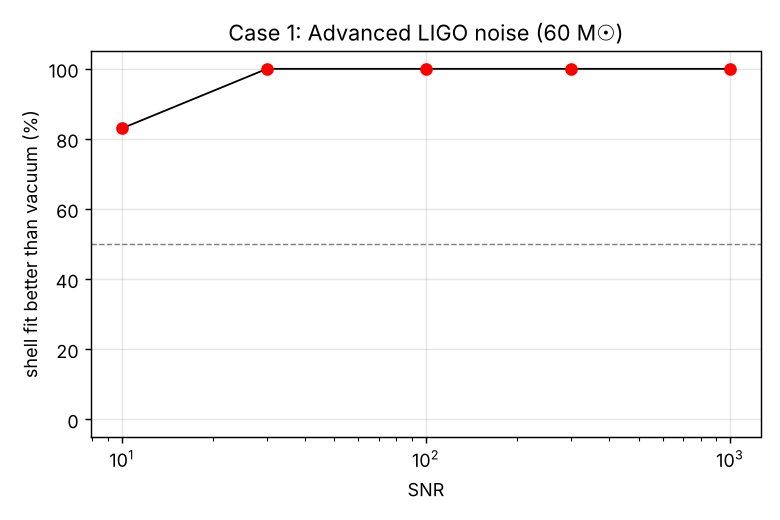
\includegraphics[width=0.32\linewidth]{plots/case_1_noise.png}
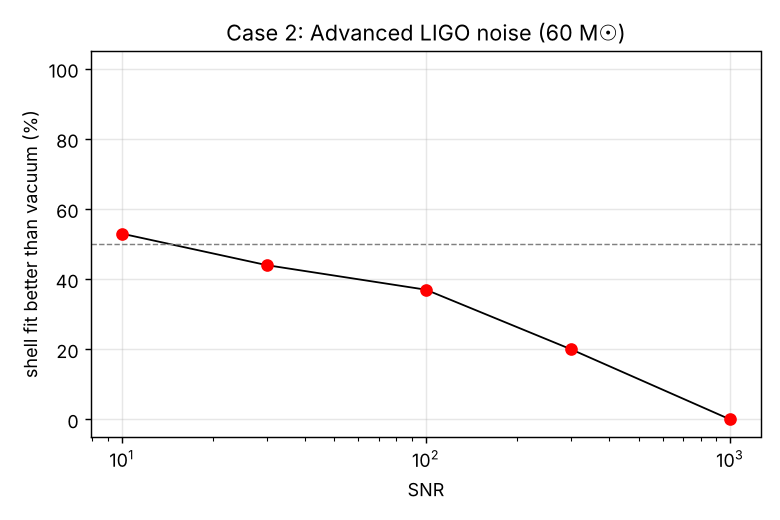
\includegraphics[width=0.32\linewidth]{plots/case_2_noise.png}
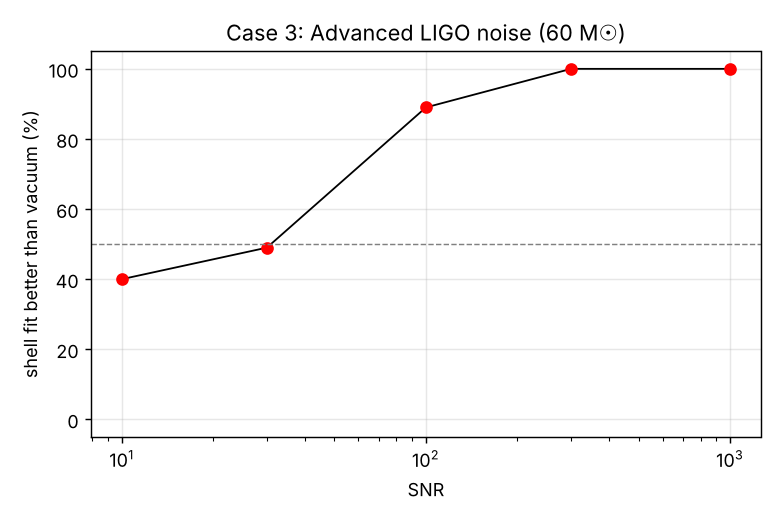
\includegraphics[width=0.32\linewidth]{plots/case_3_noise.png}
\caption{Advanced LIGO noise test (60\,$M_\odot$).}
\end{figure}

\subsection{Scan in shell mass and radius}
The three cases above are single points. To see how the result changes with the mass and the
radius of the shell, the same Advanced LIGO test is repeated on all the
coupled waveforms of the data set for which the shell modes are available: shell mass $M/2$ at
$R=6,8,10,30,45,60\,M$, $M/10$ at $R=6,8,10\,M$ and $M/100$ at $R=30,45,60\,M$. All use the same fit window,
$10$--$200\,M$ after the peak, so for the three main cases the numbers can differ slightly
from the previous section. Table~\ref{tab:scan} and Fig.~\ref{fig:scan} give the lowest SNR from which the shell
modes win in at least 90\% of the 100 realizations.


\begin{table}[H]
\centering\small
\begin{tabular}{lccccccccc}
\toprule
$\delta M$ & $R/M$ & $\alpha$ & Modes & SNR 10 & SNR 30 & SNR 100 & SNR 300 & SNR 1000 & Needed SNR \\
\midrule
$M/2$ & 6 & 1.1547 & 2 & 78\% & 100\% & 100\% & 100\% & 100\% & 30 \\
$M/2$ & 8 & 1.0954 & 3 & 63\% & 97\% & 100\% & 100\% & 100\% & 30 \\
$M/2$ & 10 & 1.0690 & 3 & 51\% & 91\% & 100\% & 100\% & 100\% & 30 \\
$M/2$ & 30 & 1.0184 & 4 & 51\% & 53\% & 89\% & 100\% & 100\% & 300 \\
$M/2$ & 45 & 1.0118 & 4 & 37\% & 35\% & 1\% & 0\% & 0\% & never \\
$M/2$ & 60 & 1.0087 & 4 & 33\% & 6\% & 0\% & 0\% & 0\% & never \\
$M/10$ & 6 & 1.0260 & 1 & 60\% & 89\% & 100\% & 100\% & 100\% & 100 \\
$M/10$ & 8 & 1.0171 & 1 & 66\% & 85\% & 100\% & 100\% & 100\% & 100 \\
$M/10$ & 10 & 1.0127 & 2 & 50\% & 65\% & 90\% & 100\% & 100\% & 100 \\
$M/100$ & 30 & 1.0004 & 4 & 32\% & 45\% & 43\% & 19\% & 0\% & never \\
$M/100$ & 45 & 1.0002 & 4 & 37\% & 37\% & 24\% & 1\% & 0\% & never \\
$M/100$ & 60 & 1.0002 & 4 & 18\% & 0\% & 0\% & 0\% & 0\% & never \\
\bottomrule
\end{tabular}
\caption{Advanced LIGO noise (60\,$M_\odot$): fraction of realizations in which the shell modes fit better, for each shell configuration.\label{tab:scan}}
\end{table}

\begin{figure}[H]
\centering
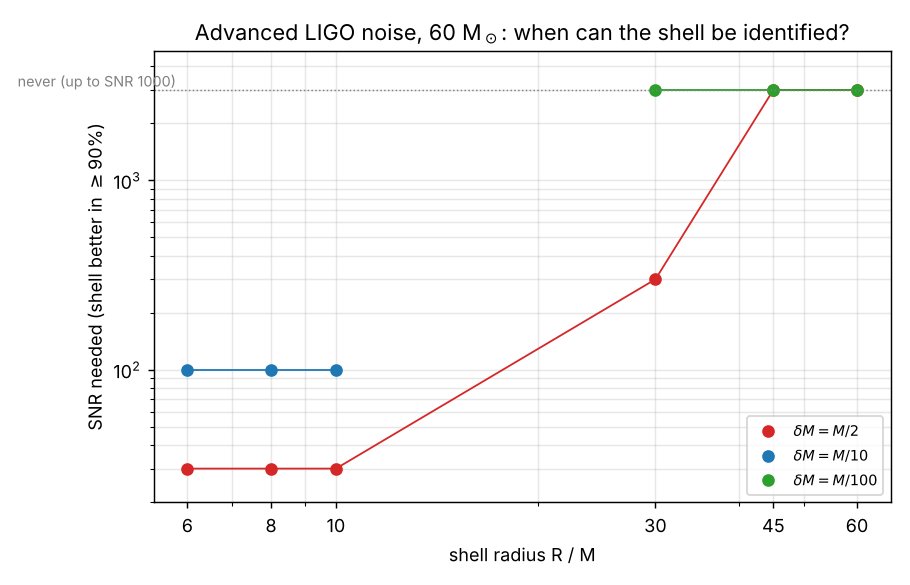
\includegraphics[width=0.6\linewidth]{plots/scan_snr_vs_radius.png}
\caption{SNR needed to identify the shell, as a function of its radius.\label{fig:scan}}
\end{figure}

\section{Summary}
\begin{itemize}
\item \textbf{Case 1} (heavy, close shell (dM = M/2, R = 6M)): best fixed-mode set shell / $\alpha$; with Advanced LIGO noise the shell modes win in at least 90\% of the realizations from SNR 30 on (at SNR 10: 83 $\pm$ 4\%).
\item \textbf{Case 2} (light, distant shell (dM = M/100, R = 30M)): best fixed-mode set vacuum; with Advanced LIGO noise the shell cannot be told apart from vacuum at any SNR studied.
\item \textbf{Case 3} (heavy, distant shell (dM = M/2, R = 30M) - echo): best fixed-mode set shell (as listed); with Advanced LIGO noise the shell modes win in at least 90\% of the realizations from SNR 300 on (at SNR 100: 89 $\pm$ 3\%).
\item \textbf{Scan}: with Advanced LIGO noise, a heavy shell ($M/2$) close to the black hole ($R\leq10M$) is identified from SNR 30 and a shell of mass $M/10$ from SNR 100; at $R=30M$ the heavy shell needs SNR 300; at $R=45M$ and $60M$, and for the light shell ($M/100$) at any radius, the shell modes never fit better than the vacuum modes.
\end{itemize}

\section{Open questions}
Which shell modes were used in the paper's fits, and are the listed shell frequencies already as seen from
infinity, or should they be divided by $\alpha$? The results with detector noise depend on the chosen mass,
which moves the ringdown frequency along the sensitivity curve; the waveform is also cut to the fit window,
so this is a simplified version of a real ringdown analysis.

At very high SNR (1000) even the shell modes no longer describe the signal completely
($\chi^2/\mathrm{ndof}=1.2$ for case 1 and 2.3 for case 3): more modes, or a separate treatment of the prompt response and of the echo, would
be needed. For distant shells ($R\geq45M$) a model with four shell modes fits worse than the vacuum modes: there
the early ringdown is vacuum-like, as found in the paper, and the shell shows up mainly in the late echo, which
would require an echo template rather than a few quasinormal modes.

\end{document}
